\section{Results}
\subsection{Code Smells}
\label{bp}
A good \AISE{} tool should only suggest code that passes code reviews by humans. We relied on the AirBNB JavaScript coding style guide~\cite{airbnb_code}, a widely used coding style and code review standard. 

The AirBNB JavaScript coding style guide contains a variety of best practices. 
Since, we are testing \cop{} for widely accepted practices and not project specific styling in JavaScript. We chose practices that were closer to design level rather than code level (e.g., logging practices rather than trailing comma use in Javascript).

Using the methodology described in Section~\ref{smells:methodology}, we picked 10 best practices in JavaScript from AirBNB JavaScript coding style guide~\cite{airbnb_code} shown in Table~\ref{tab:all_bp}. \cop{} suggested the recommended way for only one out of the ten standards we tested, i.e, Copilot did not have the recommended way as its top suggestion. Moreover, only 2 out of remaining 9 Best Practices had the Ideal way in \cop{} top 10 suggestions currently viewable. 

% \cop{} performed significantly worse than the Pythonic Idioms we showed in Section~\ref{secidioms}, As \cop{} is closed source, we cannot find the reason behind this but one could argue that lack of data for JavaScript compared to python could be a reason for this behaviour. 

Table~\ref{tab:all_bp} shows the complete list of all the Best Practices we tested on \cop{} from the AirBNB Coding Style guide~\cite{airbnb_code} and the ranking of the Ideal way in \cop{} suggestions (if it exists).

\begin{table}[ht]
    \centering
    \begin{tabular}{|L|c|}
    \hline
         \textbf{Best Practice  Title} & \textbf{\cop{} Suggestion Matched?} \\
         & (out of 10 suggestions) \\
         \hline
         Usage of Object method shorthand & No \\
         \hline
         Array Creating Constructor & 6\textsuperscript{th} \\
         \hline
         Copying Array Contents  & No \\
         \hline
         Logging a Function &  No \\
         \hline
         Exporting a Function & No \\
         \hline
         Sum of Numbers & 9\textsuperscript{th} \\
         \hline
         Accessing Properties & 1\textsuperscript{th} \\
         \hline
         Switch case usage & No \\
         \hline
         Return value from Function with a condition check & No \\
         \hline
         Converting Array-like object to an Array  & No \\
         \hline
    \end{tabular}
    \caption{List of all JavaScript Best Practices tested on \cop{}.}
    \label{tab:all_bp}
\end{table}

Figure~\ref{fig:bp_1} shows the Best Practice for Copying Array Contents, showing user input (i.e., Human Input), the top suggestion by \cop{} and the recommended way suggested by AirBNB JavaScript coding style guide~\cite{airbnb_code}.

All the Best Practices shown in Table~\ref{tab:all_bp} can be found in the \repl{} including the code used as input (i.e., Human Input), the top suggestion by \cop{} and the Ideal Way.

% \begin{tcolorbox}[title=Copying Array Contents,boxsep=.15mm]
%     %https://tex.stackexchange.com/questions/337909/tcolorbox-tcbline-style
% \textbf{Human Input:}
% \begin{lstlisting}[language=JavaScript]
% // copying array contents
% const len = items.length;
% \end{lstlisting}
% \tcbline
% \textbf{Copilot Suggestion:}
% \begin{lstlisting}[language=JavaScript]
% const copy = new Array(len);
% for (let i = 0; i < len; i++) {
% 	  copy[i] = items[i];
% }
% \end{lstlisting}
% \tcbline
% \textbf{Ideal way\footnote{source \cite{airbnb_code}}:}
% \begin{lstlisting}[language=JavaScript]
% const itemsCopy = [...items];
% \end{lstlisting}
% \end{tcolorbox}

%%%%%% TODO: remember to update the screenshot if the source citation is different from the citation in the text %%%%%%
\begin{figure}[hbt!]
    \centering
    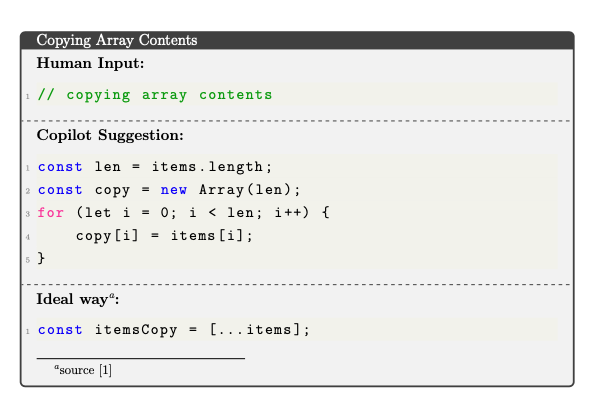
\includegraphics[width=\linewidth]{Figures/bp_1.png}
    \caption{Best Practice for Copying Array Contents amd \cop{} Suggestion.}
    \label{fig:bp_1}
\end{figure}

